\documentclass[aspectratio=169]{beamer}

\usetheme{Boadilla}
\usefonttheme{professionalfonts}
\setbeamertemplate{navigation symbols}{}
\setbeamertemplate{itemize items}[circle]
\setbeamertemplate{enumerate items}[default]
\setbeamertemplate{headline}{}

\usepackage[utf8]{inputenc}
\usepackage[T1]{fontenc}
\usepackage{lmodern}
\usepackage{amsmath}
\usepackage{booktabs}
\usepackage{tabularx}
\usepackage{array}
\usepackage{hyperref}
\usepackage[strings]{underscore}
\usepackage{listings}
\usepackage{tikz}
\usetikzlibrary{arrows.meta,positioning,fit,calc,shapes.geometric}
\usepackage{xcolor}

\definecolor{courseblue}{HTML}{12355B}
\definecolor{coursegold}{HTML}{C98A2E}
\definecolor{courseice}{HTML}{EEF3F8}
\definecolor{coursegreen}{HTML}{2F6B4F}
\definecolor{coursegray}{HTML}{4B5563}
\definecolor{codebg}{HTML}{F7F9FC}
\definecolor{codecomment}{HTML}{5E6C84}
\definecolor{codestring}{HTML}{0B6E4F}

\setbeamercolor{palette primary}{bg=courseblue,fg=white}
\setbeamercolor{palette secondary}{bg=coursegold,fg=white}
\setbeamercolor{palette tertiary}{bg=courseblue,fg=white}
\setbeamercolor{palette quaternary}{bg=coursegold,fg=white}
\setbeamercolor{structure}{fg=courseblue}
\setbeamercolor{frametitle}{bg=courseice,fg=courseblue}
\setbeamercolor{title}{fg=courseblue}
\setbeamercolor{block title}{bg=courseblue,fg=white}
\setbeamercolor{block body}{bg=courseice,fg=black}
\setbeamercolor{normal text}{fg=black,bg=white}
\setbeamercolor{alerted text}{fg=coursegold}

\setbeamerfont{footline}{size=\scriptsize}

\setbeamertemplate{footline}{
  \leavevmode
  \hbox{
    \begin{beamercolorbox}[wd=.33\paperwidth,ht=2.8ex,dp=1.2ex,leftskip=0.8em]{palette primary}%
      University of Trieste
    \end{beamercolorbox}%
    \begin{beamercolorbox}[wd=.49\paperwidth,ht=2.8ex,dp=1.2ex,center]{palette tertiary}%
      \coursename{} \textbar{} \coursecode
    \end{beamercolorbox}%
    \begin{beamercolorbox}[wd=.18\paperwidth,ht=2.8ex,dp=1.2ex,rightskip=0.8em plus1fil]{palette secondary}%
      \insertframenumber{} / \inserttotalframenumber
    \end{beamercolorbox}%
  }
}

\hypersetup{
  colorlinks=true,
  linkcolor=courseblue,
  urlcolor=coursegreen
}

\lstdefinestyle{coursepython}{
  language=Python,
  basicstyle=\ttfamily\footnotesize,
  keywordstyle=\color{courseblue}\bfseries,
  commentstyle=\color{codecomment}\itshape,
  stringstyle=\color{codestring},
  showstringspaces=false,
  columns=fullflexible,
  keepspaces=true,
  frame=single,
  framerule=0.6pt,
  rulecolor=\color{courseblue},
  backgroundcolor=\color{codebg},
  xleftmargin=0.4em,
  xrightmargin=0.4em,
  aboveskip=0.4em,
  belowskip=0.2em
}

\newcommand{\coursename}{Data-driven Systems Engineering}
\newcommand{\coursecode}{440MI / 305SM}
\newcommand{\coursefooter}{}

\newcommand{\learninggoals}[1]{
  \begin{block}{Learning goals}
  #1
  \end{block}
}

\newcommand{\repoactivity}[1]{
  \begin{block}{Repo activity}
  #1
  \end{block}
}

\newcommand{\readinglist}[1]{
  \begin{block}{Papers and materials}
  {\footnotesize #1}
  \end{block}
}

\newcommand{\coursecontextframe}[5]{
  \begin{frame}{Course Map and Running Cases}
  \centering
  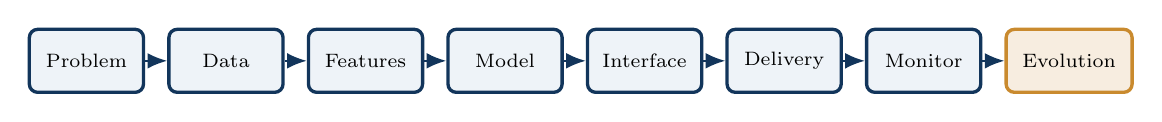
\begin{tikzpicture}[node distance=0.28cm]
  \node[flowbox, minimum width=1.45cm, minimum height=0.8cm] (problem) {\scriptsize Problem};
  \node[flowbox, minimum width=1.45cm, minimum height=0.8cm, right=of problem] (data) {\scriptsize Data};
  \node[flowbox, minimum width=1.45cm, minimum height=0.8cm, right=of data] (features) {\scriptsize Features};
  \node[flowbox, minimum width=1.45cm, minimum height=0.8cm, right=of features] (model) {\scriptsize Model};
  \node[flowbox, minimum width=1.45cm, minimum height=0.8cm, right=of model] (interface) {\scriptsize Interface};
  \node[flowbox, minimum width=1.45cm, minimum height=0.8cm, right=of interface] (delivery) {\scriptsize Delivery};
  \node[flowbox, minimum width=1.45cm, minimum height=0.8cm, right=of delivery] (monitor) {\scriptsize Monitor};
  \node[accentbox, minimum width=1.6cm, minimum height=0.8cm, right=of monitor] (evolution) {\scriptsize Evolution};
  \foreach \a/\b in {problem/data,data/features,features/model,model/interface,interface/delivery,delivery/monitor,monitor/evolution} {
    \draw[arrow] (\a) -- (\b);
  }
  \end{tikzpicture}

  \vspace{0.5em}
  \begin{block}{Today in the course}
  \textbf{Focus:} #1

  \textbf{Bridge:} #2
  \end{block}

  \begin{columns}[T]
  \column{0.48\textwidth}
  \begin{block}{Fraud case}
  {\footnotesize #3}
  \end{block}
  \column{0.48\textwidth}
  \begin{block}{Pasteurization case}
  {\footnotesize #4}
  \end{block}
  \end{columns}

  \vspace{0.3em}
  {\footnotesize \textbf{Course thread:} #5}
  \coursefooter
  \end{frame}
}

\newcommand{\classclosingframe}[4]{
  \begin{frame}{From This Class to the Next}
  \begin{block}{What stays with us}
  #1
  \end{block}

  \begin{columns}[T]
  \column{0.48\textwidth}
  \begin{block}{Project use}
  {\footnotesize #2}
  \end{block}
  \column{0.48\textwidth}
  \begin{block}{Next connection}
  {\footnotesize #3}
  \end{block}
  \end{columns}

  \vspace{0.3em}
  {\footnotesize \textbf{Course thread:} #4}
  \coursefooter
  \end{frame}
}

\tikzset{
  flowbox/.style={
    rounded corners=3pt,
    draw=courseblue,
    fill=courseice,
    very thick,
    minimum width=2.2cm,
    minimum height=0.9cm,
    align=center,
    font=\small
  },
  accentbox/.style={
    rounded corners=3pt,
    draw=coursegold,
    fill=coursegold!15,
    very thick,
    minimum width=2.2cm,
    minimum height=0.9cm,
    align=center,
    font=\small
  },
  arrow/.style={
    -{Latex[length=2.5mm,width=2mm]},
    thick,
    draw=courseblue
  }
}


\title{Class 9: Dealing with Data --- pandas Basics}
\author{\coursename}
\date{}

\begin{document}

\frame{\titlepage \coursefooter}

\begin{frame}{Agenda}
\begin{itemize}
\item Loading a dataset and understanding the pandas Index.
\item Selecting rows and columns: \texttt{loc}, \texttt{iloc}, and boolean filters.
\item Renaming and dropping columns for clarity.
\item Categorical summaries and grouped statistics.
\item Where ``cleaning'' ends and feature engineering begins.
\end{itemize}
\coursefooter
\end{frame}

\begin{frame}{Learning goals}
\learninggoals{
\begin{itemize}
\item Load a dataset and inspect its structure, types, and missingness.
\item Select data precisely using label-based, position-based, and boolean access.
\item Rename and drop columns to make a DataFrame easier to work with.
\item Summarize a categorical column and compute grouped statistics.
\item Explain the boundary between pandas-level cleaning and feature engineering.
\end{itemize}
}
\coursefooter
\end{frame}

\coursecontextframe
{pandas mechanics for loading, indexing, and lightly cleaning a dataset.}
{Class 6 got data into a DataFrame; this class is about handling that DataFrame with precision before anything gets modeled.}
{The fraud dataset's target column arrives named \texttt{Class}; renaming it to \texttt{is\_fraud} and separating it from the features is pandas mechanics, not modeling.}
{The pasteurization case eventually needs the same discipline: consistent column names and dtypes before any sensor batch can be trusted.}
{This class deliberately stops at cleaning. Deciding which features to derive or transform is data-theory work, picked up later in the Data-Driven block.}

\begin{frame}[fragile]{Loading and a first look}
\begin{lstlisting}[style=coursepython]
iris = sns.load_dataset("iris")
iris.head()
iris.info()
\end{lstlisting}
\begin{itemize}
\item From `notebooks/Class2\_EDA.ipynb`: \texttt{iris} is a DataFrame with columns \texttt{sepal\_length}, \texttt{sepal\_width}, \texttt{petal\_length}, \texttt{petal\_width}, and \texttt{species}.
\item Every DataFrame carries a row \textbf{Index} alongside its columns --- by default, integers starting at 0.
\item \texttt{.info()} reports the dtype of every column: four \texttt{float64} columns and one \texttt{object} column here.
\end{itemize}
\coursefooter
\end{frame}

\begin{frame}[fragile]{Checking for missing values}
\begin{lstlisting}[style=coursepython]
iris.isnull().sum()
\end{lstlisting}
\begin{itemize}
\item Also from `Class2\_EDA.ipynb`: this turns ``is anything missing?'' into one concrete number per column.
\item Iris happens to be clean --- every count is zero --- but the habit matters more than this particular answer.
\item The fraud dataset needs the same check before its 30-plus columns are trusted for anything.
\end{itemize}
\coursefooter
\end{frame}

\begin{frame}[fragile]{Selecting with \texttt{loc} and \texttt{iloc}}
\begin{lstlisting}[style=coursepython]
iris.loc[0, "species"]        # label-based: row label 0, column "species"
iris.iloc[0, 4]                # position-based: first row, fifth column
iris.loc[:, ["species", "petal_length"]]   # a subset of columns
\end{lstlisting}
\begin{itemize}
\item \texttt{.loc} indexes by label (row label and column name); \texttt{.iloc} indexes by integer position, regardless of label.
\item For a DataFrame with the default integer index, label and position often coincide for rows --- but they are not the same concept, and a filtered DataFrame makes the difference obvious.
\end{itemize}
\coursefooter
\end{frame}

\begin{frame}[fragile]{Boolean filtering}
\begin{lstlisting}[style=coursepython]
setosa_only = iris[iris["species"] == "setosa"]
large_petals = iris[iris["petal_length"] > 5.0]
\end{lstlisting}
\begin{itemize}
\item A boolean expression inside \texttt{df[...]} keeps only the rows where the condition is true.
\item This is the single most common way to answer ``show me the subset where...'' in pandas.
\item The same pattern isolates fraud cases in the credit-card dataset, or a single process state in the pasteurization data.
\end{itemize}
\coursefooter
\end{frame}

\begin{frame}[fragile]{Renaming and dropping columns}
\begin{lstlisting}[style=coursepython]
df.rename(columns={'Class': 'is_fraud'}, inplace=True)

X = df.drop('is_fraud', axis=1)
y = df['is_fraud']
\end{lstlisting}
\begin{itemize}
\item From `streamlit/modeling.py`: the raw dataset calls its target \texttt{Class}; renaming it to \texttt{is\_fraud} makes every later line more readable.
\item \texttt{inplace=True} modifies \texttt{df} directly instead of returning a new, renamed copy.
\item Splitting a target out with \texttt{.drop()} and \texttt{[...]} is still pandas mechanics --- deciding \emph{which columns to keep} as features is feature engineering, not this class.
\end{itemize}
\coursefooter
\end{frame}

\begin{frame}[fragile]{Categorical summaries}
\begin{lstlisting}[style=coursepython]
iris["species"].value_counts()
\end{lstlisting}
\begin{itemize}
\item From `Class2\_EDA.ipynb`: one line that turns a categorical column into a count per category.
\item For iris the classes are balanced (50 each); for the fraud target, the same call reveals a dataset that is almost entirely non-fraud --- a fact any later modeling decision has to respect.
\end{itemize}
\coursefooter
\end{frame}

\begin{frame}[fragile]{Grouped statistics}
\begin{lstlisting}[style=coursepython]
iris.groupby("species").describe().T
\end{lstlisting}
\begin{itemize}
\item Also from `Class2\_EDA.ipynb`: \texttt{groupby} splits the DataFrame by category, then \texttt{.describe()} summarizes each group separately.
\item \texttt{.T} transposes the result so species become columns and statistics become rows --- purely a readability choice.
\item This single line already tells you more than a global \texttt{.describe()} ever could, without touching a model.
\end{itemize}
\coursefooter
\end{frame}

\begin{frame}{Duplicates and obvious dtype fixes}
\begin{itemize}
\item \texttt{df.duplicated()} flags exact-duplicate rows; \texttt{df.drop\_duplicates()} removes them.
\item \texttt{df["col"].astype(...)} fixes a column stuck in the wrong dtype, for example a numeric column read in as text.
\item These are still mechanical fixes: they correct how the data is represented, not what the data should mean for a model.
\item Always check row counts before and after --- a silent drop of ``duplicate'' rows that are not really duplicates is a common mistake.
\end{itemize}
\coursefooter
\end{frame}

\begin{frame}{Cleaning versus feature engineering: where this class stops}
\begin{tabularx}{\textwidth}{>{\bfseries}l X}
This class (cleaning) & The Data-Driven block (feature engineering) \\
\toprule
Renaming a confusing column & Deciding which columns become model inputs \\
Checking and handling missing values & Imputation strategy and its trade-offs \\
Fixing an obviously wrong dtype & Encoding, scaling, and transformation choices \\
Dropping an exact duplicate row & Deriving new columns from existing ones \\
\bottomrule
\end{tabularx}
\vspace{0.4em}
\begin{itemize}
\item Everything on the left is pandas mechanics; everything on the right is a modeling decision with theory behind it.
\end{itemize}
\coursefooter
\end{frame}

\begin{frame}{How the repo already uses today's building blocks}
\repoactivity{
\begin{itemize}
\item `notebooks/Class2\_EDA.ipynb` runs \texttt{.head()}, \texttt{.info()}, \texttt{.isnull().sum()}, \texttt{.value\_counts()}, and \texttt{.groupby(...).describe()} on the iris dataset in sequence.
\item `streamlit/modeling.py` renames the fraud target column before ever splitting features from labels.
\item Open the notebook and identify which of today's five operations appears in which cell.
\end{itemize}
}
\coursefooter
\end{frame}

\begin{frame}{Discussion prompt}
\begin{block}{Question}
`value_counts()` on the fraud target shows a dataset that is almost entirely non-fraud. Is that a data-cleaning problem, a feature-engineering problem, or neither?
\end{block}
\begin{itemize}
\item Deliberately has no clean answer yet --- it previews why class imbalance gets its own treatment later in the Data-Driven block.
\end{itemize}
\coursefooter
\end{frame}

\begin{frame}{Papers and materials}
\readinglist{
\href{https://pandas.pydata.org/docs/}{pandas documentation};\
\href{https://pandas.pydata.org/docs/getting_started/overview.html}{pandas overview};\
\href{https://hdsr.mitpress.mit.edu/pub/9ymoz9h7}{Sambasivan et al.\ (2021), Everyone wants to do the model work, not the data work}.
}
\coursefooter
\end{frame}

\classclosingframe
{\begin{itemize}
\item \texttt{loc}, \texttt{iloc}, and boolean filters cover almost every ``give me this subset'' question you will ask of a DataFrame.
\item Renaming, dropping, and checking dtypes are cleaning; deciding what a feature should be is a different, later decision.
\item `Class2\_EDA.ipynb` and `modeling.py` already show every operation from today in a real dataset.
\end{itemize}}
{Any project step that starts with ``first, load and clean the data'' is exactly today's material, no more and no less.
}
{Class 10 uses these same habits to run a full exploratory data analysis, this time reading plots as well as tables.}
{Clean, well-indexed data is what makes the next class's plots worth trusting.}

\end{document}
